\newcommand{\thetm}{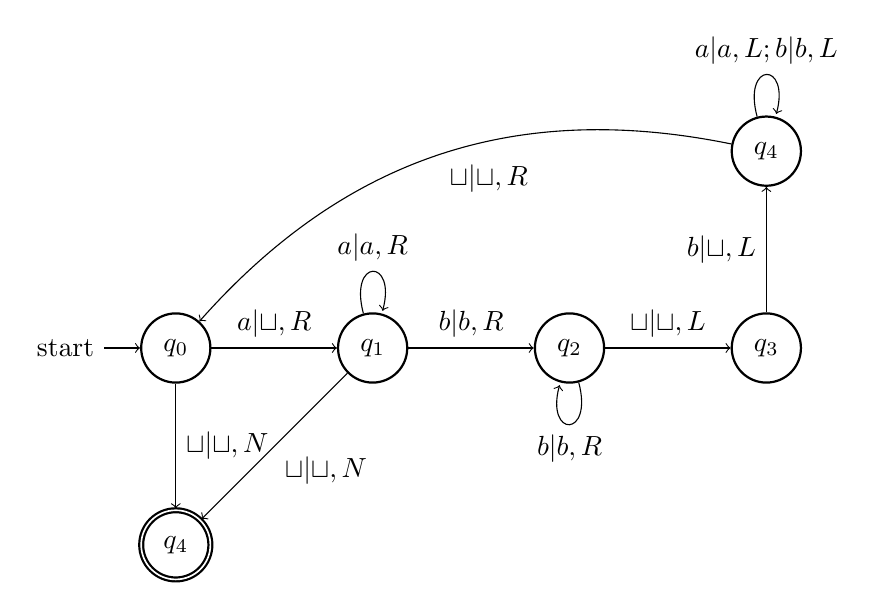
\begin{tikzpicture}[node distance=2.5cm,auto]
  \node(q0)[state,initial]{$q_0$};
  \node(q1)[state,right of=q0]{$q_1$};
  \node(q2)[state,right of=q1]{$q_2$};
  \node(q3)[state,right of=q2]{$q_3$};
  \node(q4)[state,above of=q3]{$q_4$};
  \node(q5)[state,accepting,below of=q0]{$q_4$};
  \path[->]       (q0) edge node{$a|\sqcup,R$} (q1)
	          (q0) edge node{$\sqcup|\sqcup,N$} (q5)
	          (q1) edge[loop above] node{$a|a,R$} ()
	          (q1) edge node{$b|b,R$} (q2)
	          (q1) edge node{$\sqcup|\sqcup,N$} (q5)
	          (q2) edge[loop below] node{$b|b,R$} ()
	          (q2) edge node{$\sqcup|\sqcup,L$} (q3)
	          (q3) edge node{$b|\sqcup,L$} (q4)
	          (q4) edge[loop above] node{$a|a,L; b|b,L$} ()
	          (q4) edge[bend right] node{$\sqcup|\sqcup,R$} (q0);
 \end{tikzpicture}}

\documentclass[t]{beamer}
\usetheme[deutsch]{KIT}
\setbeamercovered{transparent}
\setbeamertemplate{navigation symbols}{}

\KITfoot{Tutoriumsmaterial von Michael Fuerst}
\usepackage[utf8]{inputenc}
\usepackage{amsmath}
\usepackage{ifthen}
\usepackage{amssymb}
\usepackage{tikz}
\usepackage{ngerman}
\usepackage[normalem]{ulem}
\usepackage{stmaryrd}
\usetikzlibrary{automata}
\usenavigationsymbols


\title{Theoretische Grundlagen der Informatik}
\subtitle{Tutorium}
\author{Michael Fuerst}

\institute[IKS]{Institut für Theoretische Informatik}

\TitleImage[height=\titleimageht]{images/tmaschine.png}

\newcommand{\N}{\ensuremath{\mathbb{N}}}
\newcommand{\M}{\ensuremath{\mathcal{M}}}
\newcommand{\classP}{\ensuremath{\mathcal{P}}}
\newcommand{\classNP}{\ensuremath{\mathcal{NP}}}
\newcommand{\co}{\ensuremath{\mathsf{co\text{-}}}}
\newcommand{\pot}{\ensuremath{\mathcal{P}}}
\newcommand{\abs}[1]{\ensuremath{\left\vert #1 \right\vert}}
\newcommand{\menge}[2]{\ensuremath{\left\lbrace #1 \,\middle\vert\, #2 \right\rbrace}}
\newcommand{\ducttape}[1]{\vspace{#1}}
\newcommand{\neglit}[1]{\overline{#1\vphantom{x^a}}}
\newcommand{\recipe}{\raisebox{-.3cm}{
\includegraphics[scale=.15]{images/chefs-cap.png}}\hspace{0.2cm}}
\newcommand{\opt}[1]{\ensuremath{\text{OPT}(#1)}}
\newcommand{\A}[1]{\ensuremath{\mathcal{A}(#1)}}
\renewcommand{\O}[1]{\ensuremath{\mathcal{O}(#1)}}
\newcommand{\msout}[1]{\text{\sout{\ensuremath{#1}}}}

\newcommand{\invincible}{\setbeamercovered{invisible}} %  "Yesss! I am invincible!!" (Boris Grishenko)
\newcommand{\vincible}{\setbeamercovered{transparent}}
\renewcommand{\solution}[1]{\invincible \pause #1 \vincible}
\newcommand{\micropause}{\\[8pt]}

% \@ifundefined{tikzset}{}{\tikzset{initial text=}} % Text "start" bei Startknoten unterdrücken
\tikzstyle{every node}=[thick]
\tikzstyle{every line}=[thick]

\newcommand{\tutnr}[1]{
  \subtitle{Tutorium #1}
	\begin{frame}
		\maketitle
	\end{frame}
}

\newcommand{\uebnr}[1]{
  \subtitle{Anmerkungen zum #1. Übungsblatt}
	\begin{frame}
		\maketitle
	\end{frame}
}

\begin{document}

\tutnr{13}

\section{Entscheidbarkeit}
\subsection{Entscheidbarkeit}
\begin{frame}
 \frametitle{Definitionen zur TM (Vorlesung)}
 \begin{enumerate}
  \item Eine TM \emph{akzeptiert} eine Eingabe $w \in \Sigma^*$, wenn sie nach Lesen von $w$ in einem Zustand aus $F$ stoppt.
  \item Sie \emph{akzeptiert} eine Sprache $L \subseteq \Sigma^*$, wenn sie genau die Wörter $w$ aus $L$ als Eingabe akzeptiert.
\end{enumerate}
\end{frame}
\begin{frame}
 \frametitle{Definitionen zur TM (Vorlesung)}
 \begin{enumerate}
 \setcounter{enumi}{2}
 \item Eine Sprache $L \subseteq \Sigma^*$ heißt \emph{rekursiv} oder \emph{entscheidbar}, wenn es eine Turingmaschine gibt, die auf allen Eingaben stoppt und
	ein Wort $w \in \Sigma^*$ genau dann akzeptiert, wenn $w \in L$ gilt.
  \item Eine Sprache $L \subseteq \Sigma^*$ heißt \emph{rekursiv-aufzählbar} oder \emph{semi-entscheidbar}, wenn es eine Turingmaschine gibt, die ein Wort $w \in \Sigma^*$ genau dann akzeptiert, wenn $w \in L$ gilt. \\ Das Verhalten der Turingmaschine für Eingaben $w \not\in L$ ist damit nicht definiert.
	Sie stoppt entweder nicht in einem Endzustand oder aber stoppt gar nicht.
	\item Eine TM \emph{realisiert} die Funktion $f: \Sigma^* \rightarrow \Gamma^*$ mit $$f(w) = \begin{cases} \text{Ausgabe der TM nach Abarbeitung von } w & \text{wenn die TM hält} \\ \text{undefiniert} & \text{sonst} \end{cases}$$
 \end{enumerate}
\end{frame}

\begin{frame}
 \frametitle{Beispiel zur Akzeptanz}
 \begin{itemize}
  \item $\Sigma := \{a, b\}$  
  \item $F := \{q_4\}$
  
  \ducttape{-1cm} 
  \thetm
 \end{itemize}
 
 \end{frame}

\begin{frame}
 \frametitle{Sprache}
 \begin{itemize}
  \item $aab$ wird von der TM akzeptiert.
  \item $abb$ nicht.
  \item Die akzeptierte Sprache ist $L(TM) := \menge{a^kb^l}{k \geq l}$
 

 \hfill 
 \resizebox{8cm}{!} {%
  \thetm
 }
  \invincible
  \pause
 \ducttape{-6cm} 
  \vincible
 \end{itemize}
 
\end{frame}

\subsection{Halteproblem}
\begin{frame}
	\frametitle{Halteproblem}.
	Das Halteproblem beschreibt die Aufgabe zu entscheiden, ob eine Turingmaschine bei gegeben Eingabewort hält oder nicht. Dieses Problem ist im allgemeinen Fall semi-entscheidbar, aber nicht entscheidbar.~\\~\\
	\begin{itemize}
		\item Formal: $(\langle M\rangle, w) \in HALT \Leftrightarrow M \text{ hält bei der Eingabe } w$
	\end{itemize}
\end{frame}

\begin{frame}
	\frametitle{Aufgabe zur Entscheidbarkeit}
	
	Sei $L$ eine nicht entscheidbare Sprache \"uber dem Alphabet $\Sigma=\{0,1\}$ und sei $(01)^k \not\in L$ f\"ur jedes $k\in \mathbb N_{>0}$.
	
Zeige: Die Sprache \[L' = \{w_1\#w_2\mid (w_1 \in L \wedge w_2 \not\in L) \text{ oder } (w_1 \not\in L \wedge w_2 \in L) \}\]
\"uber dem Alphabet $\Sigma'=\{0, 1, \#\}$ ist nicht entscheidbar.

	\invincible \pause
	
	\ducttape{1cm}	
	
	\only<2-3>{
Annahme: $L'$ ist entscheidbar. Sei $M'$ dann eine Turingmaschine, die $L'$ entscheidet. $M'$ entscheidet also zun\"achst, ob der erste Teil des Wortes in $L$ liegt, und dann, ob der zweite Teil des Wortes nicht in $L$ liegt.

Sei $M$ eine Turingmaschine, die die erste Phase von $M'$ simuliert. Dann entscheidet $M$ die Sprache $L$, was ein Widerspruch zur Annahme ist.

	\pause
	\begin{center}
        \Huge{\textbf{\color{red}NOPE}}
    \end{center}
	
	}

	\only<4>{	
	Annahme: $L'$ ist entscheidbar. 
Sei $M'$ eine TM, die $L'$ entscheidet.
F\"ur ein Wort $w \in \Sigma^*$ konstruiere das Wort $w'=w\#01$. 
Dann gilt: $w' \in L' \Leftrightarrow w \in L$. 

Damit kann man $L$ wie folgt entscheiden, im Widerspruch zur Nichtentscheidbarkeit von $L$:\\
%F\"ur $w \in \Sigma^*$ konstruiere $w'=w\#01$.
Simuliere die TM $M'$ auf Eingabe $w'$ und akzeptiere $w \in L$ gdw. $M'$ $w' \in L'$ akzeptiert.
	}

	\vincible
	
\end{frame}

\subsection{Tut 1314 - Beispiel B5 A4}
\begin{frame}
	\frametitle{Beispielaufgabe Entscheidbarkeit (B5 A4)}
	Zeigen Sie, dass die Sprache \\ $\mathcal{L} = \{ \langle \mathcal{M} \rangle \; | \; \mbox{Turingmaschine $\mathcal{M}$ akzeptiert jede Eingabe} \}$ \\ nicht entscheidbar ist!
\end{frame}
\subsection{Tut 1314 - Aufgabe B6 A1}
\begin{frame}
	\frametitle{Aufgabe B6 A1}
	Zeigen Sie, dass die Sprache \\ $\mathcal{L} = \{\langle\mathcal{M}\rangle \; | \; \mbox{Turingmaschine $\mathcal{M}$ hat mindestens einen unerreichbaren Zustand}\}$ \\ nicht entscheidbar ist!
\end{frame}

\subsection{Tut 1314 - Aufgabe B6 A3}
\begin{frame}
	\frametitle{Aufgabe B6 A3 rekursiv aufzählbare Mengen}
	Welche der folgenden Mengen sind rekursiv aufz"ahlbar? \\
	Beweisen Sie Ihre Aussage!
	\begin{enumerate}
		\item $M_1 := \{q \in \mathbb{Q} \; | \; 0<q<1\}$
		\item $M_2 := \{r \in \mathbb{R} \; | \; 0<r<1\}$
	\end{enumerate}
\end{frame}

\section{Satz von Rice}
\subsection{Satz von Rice}
\begin{frame}
\frametitle{Satz von Rice}
Der Satz von Rice sagt aus, dass es unmöglich ist, eine nichttriviale Eigenschaft von Turingmaschinen algorithmisch zu entscheiden.
\begin{block}{Formale Version}
Es sei $R$ die Klasse aller Turing-berechenbaren Funktionen und $S$ eine beliebige nichttriviale (das bedeutet $S \neq \emptyset$ und $S \neq R$) Teilmenge davon. Dann ist die Sprache
$$ C_S = \menge{M}{M \text{ realisiert eine Funktion aus } S} $$
unentscheidbar. 
\end{block}
\end{frame}
% Beispiel
\begin{frame}
\frametitle{Beispiel}
Die Klasse aller Programme, die etwas auf einem Rechner tun, das der Benutzer nicht möchte (das ist eine Teilmenge der turing-berechenbaren Funktionen) ist unentscheidbar. Daraus folgt, dass es keinen perfekten Virenscanner geben kann!
\end{frame}

\begin{frame}
\frametitle{Aufgabe: Entscheidbarkeit}
\begin{enumerate}
\item Zeige, dass die Sprache $$L_{\emptyset} := \{\langle \mathcal M \rangle \mid \mathcal M \text{ Turingmaschine}, L(\mathcal M) = \emptyset\}$$ nicht entscheidbar ist.
\end{enumerate}
\end{frame}

% Aufgabe
\begin{frame}
\frametitle{Aufgabe}
Kann man die Entscheidbarkeit der folgenden Mengen mithilfe des Satzes von Rice bestimmen?
\begin{itemize}
\item Alle Turingmaschinen, die bei Eingabe des leeren Wortes nur $0$ aufs Band schreiben.
\item Alle Turingmaschinen, die im ersten Schritt genau eine $0$ aufs Band schreiben und im zweiten Schritt anhalten. 
\item Alle Turingmaschinen, die bei Eingabe des leeren Wortes das Band irgendwann einmal verändern.
\end{itemize}
\end{frame}

\section{Klausuraufgaben}
\subsection{Dynamische Programmierung}
\begin{frame}
\frametitle{Klausur 0405 Aufgabe 3 b}
(Siehe Klausur.)
\end{frame}

\subsection{Integer Programming}
\begin{frame}
\frametitle{Klausur 0304 Aufgabe 3 b}
(Siehe Klausur.)
\end{frame}

\subsection{Weitere Klausuraufgaben}
\begin{frame}
\frametitle{Beliebige Klausuraufgaben}
(Siehe Klausur.)
\end{frame}

\section{Schluss}
\subsection{Schluss}
\begin{frame}
	\frametitle{Bis zum nächsten Mal!}
    \begin{center}
        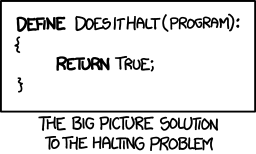
\includegraphics[width=\textwidth]{images/halting_problem.png}
    \end{center}
\end{frame}

\frame{
  \frametitle{Lizenzen}
  \center
  
\includegraphics[width=2em]{images/by}
  
\includegraphics[width=2em]{images/cc}
  
\includegraphics[width=2em]{images/sa}
  \\
  {\tiny

Dieses Werk ist unter einem ``Creative Commons Namensnennung-Weitergabe unter gleichen Bedingungen 3.0 Deutschland``-Lizenzvertrag lizenziert. Um eine Kopie der Lizenz zu erhalten, gehen Sie bitte zu \href{http://creativecommons.org/licenses/by-sa/3.0/de/}{http://creativecommons.org/licenses/by-sa/3.0/de/} oder schreiben Sie an Creative Commons, 171 Second Street, Suite 300, San Francisco, California 94105, USA.\\
  \vspace{1cm}
  Davon ausgenommen sind das Titelbild, welches aus der März-April 2002 Ausgabe von American Scientist erschienen ist und ohne Erlaubnis verwendet wird, sowie das KIT Beamer Theme. Hierfür gelten die Bestimmungen der jeweiligen Urheber.
  \vspace{1cm}
  \\ 
  }
  %Habe hier die Reihenfolge etwas umgestellt, weil die Formatierung bei mir komisch aussah. 
  %Wenn es bei dir anders ist, kannst du es auch wieder zurückändern, dann haben wir unterschiedliche Kompilieroptionen
}

\end{document}
